\PassOptionsToPackage{unicode=true}{hyperref} % options for packages loaded elsewhere
\PassOptionsToPackage{hyphens}{url}
%
\documentclass[
]{article}
\usepackage{lmodern}
\usepackage{amssymb,amsmath}
\usepackage{ifxetex,ifluatex}
\ifnum 0\ifxetex 1\fi\ifluatex 1\fi=0 % if pdftex
  \usepackage[T1]{fontenc}
  \usepackage[utf8]{inputenc}
  \usepackage{textcomp} % provides euro and other symbols
\else % if luatex or xelatex
  \usepackage{unicode-math}
  \defaultfontfeatures{Scale=MatchLowercase}
  \defaultfontfeatures[\rmfamily]{Ligatures=TeX,Scale=1}
  \setmainfont[]{Verdana}
\fi
% use upquote if available, for straight quotes in verbatim environments
\IfFileExists{upquote.sty}{\usepackage{upquote}}{}
\IfFileExists{microtype.sty}{% use microtype if available
  \usepackage[]{microtype}
  \UseMicrotypeSet[protrusion]{basicmath} % disable protrusion for tt fonts
}{}
\makeatletter
\@ifundefined{KOMAClassName}{% if non-KOMA class
  \IfFileExists{parskip.sty}{%
    \usepackage{parskip}
  }{% else
    \setlength{\parindent}{0pt}
    \setlength{\parskip}{6pt plus 2pt minus 1pt}}
}{% if KOMA class
  \KOMAoptions{parskip=half}}
\makeatother
\usepackage{xcolor}
\IfFileExists{xurl.sty}{\usepackage{xurl}}{} % add URL line breaks if available
\IfFileExists{bookmark.sty}{\usepackage{bookmark}}{\usepackage{hyperref}}
\hypersetup{
  pdftitle={Formatting, Latex, plot and table samples},
  pdfauthor={Fabian Koch},
  pdfborder={0 0 0},
  breaklinks=true}
\urlstyle{same}  % don't use monospace font for urls
\usepackage[margin=1in]{geometry}
\usepackage{color}
\usepackage{fancyvrb}
\newcommand{\VerbBar}{|}
\newcommand{\VERB}{\Verb[commandchars=\\\{\}]}
\DefineVerbatimEnvironment{Highlighting}{Verbatim}{commandchars=\\\{\}}
% Add ',fontsize=\small' for more characters per line
\usepackage{framed}
\definecolor{shadecolor}{RGB}{248,248,248}
\newenvironment{Shaded}{\begin{snugshade}}{\end{snugshade}}
\newcommand{\AlertTok}[1]{\textcolor[rgb]{0.94,0.16,0.16}{#1}}
\newcommand{\AnnotationTok}[1]{\textcolor[rgb]{0.56,0.35,0.01}{\textbf{\textit{#1}}}}
\newcommand{\AttributeTok}[1]{\textcolor[rgb]{0.77,0.63,0.00}{#1}}
\newcommand{\BaseNTok}[1]{\textcolor[rgb]{0.00,0.00,0.81}{#1}}
\newcommand{\BuiltInTok}[1]{#1}
\newcommand{\CharTok}[1]{\textcolor[rgb]{0.31,0.60,0.02}{#1}}
\newcommand{\CommentTok}[1]{\textcolor[rgb]{0.56,0.35,0.01}{\textit{#1}}}
\newcommand{\CommentVarTok}[1]{\textcolor[rgb]{0.56,0.35,0.01}{\textbf{\textit{#1}}}}
\newcommand{\ConstantTok}[1]{\textcolor[rgb]{0.00,0.00,0.00}{#1}}
\newcommand{\ControlFlowTok}[1]{\textcolor[rgb]{0.13,0.29,0.53}{\textbf{#1}}}
\newcommand{\DataTypeTok}[1]{\textcolor[rgb]{0.13,0.29,0.53}{#1}}
\newcommand{\DecValTok}[1]{\textcolor[rgb]{0.00,0.00,0.81}{#1}}
\newcommand{\DocumentationTok}[1]{\textcolor[rgb]{0.56,0.35,0.01}{\textbf{\textit{#1}}}}
\newcommand{\ErrorTok}[1]{\textcolor[rgb]{0.64,0.00,0.00}{\textbf{#1}}}
\newcommand{\ExtensionTok}[1]{#1}
\newcommand{\FloatTok}[1]{\textcolor[rgb]{0.00,0.00,0.81}{#1}}
\newcommand{\FunctionTok}[1]{\textcolor[rgb]{0.00,0.00,0.00}{#1}}
\newcommand{\ImportTok}[1]{#1}
\newcommand{\InformationTok}[1]{\textcolor[rgb]{0.56,0.35,0.01}{\textbf{\textit{#1}}}}
\newcommand{\KeywordTok}[1]{\textcolor[rgb]{0.13,0.29,0.53}{\textbf{#1}}}
\newcommand{\NormalTok}[1]{#1}
\newcommand{\OperatorTok}[1]{\textcolor[rgb]{0.81,0.36,0.00}{\textbf{#1}}}
\newcommand{\OtherTok}[1]{\textcolor[rgb]{0.56,0.35,0.01}{#1}}
\newcommand{\PreprocessorTok}[1]{\textcolor[rgb]{0.56,0.35,0.01}{\textit{#1}}}
\newcommand{\RegionMarkerTok}[1]{#1}
\newcommand{\SpecialCharTok}[1]{\textcolor[rgb]{0.00,0.00,0.00}{#1}}
\newcommand{\SpecialStringTok}[1]{\textcolor[rgb]{0.31,0.60,0.02}{#1}}
\newcommand{\StringTok}[1]{\textcolor[rgb]{0.31,0.60,0.02}{#1}}
\newcommand{\VariableTok}[1]{\textcolor[rgb]{0.00,0.00,0.00}{#1}}
\newcommand{\VerbatimStringTok}[1]{\textcolor[rgb]{0.31,0.60,0.02}{#1}}
\newcommand{\WarningTok}[1]{\textcolor[rgb]{0.56,0.35,0.01}{\textbf{\textit{#1}}}}
\usepackage{graphicx,grffile}
\makeatletter
\def\maxwidth{\ifdim\Gin@nat@width>\linewidth\linewidth\else\Gin@nat@width\fi}
\def\maxheight{\ifdim\Gin@nat@height>\textheight\textheight\else\Gin@nat@height\fi}
\makeatother
% Scale images if necessary, so that they will not overflow the page
% margins by default, and it is still possible to overwrite the defaults
% using explicit options in \includegraphics[width, height, ...]{}
\setkeys{Gin}{width=\maxwidth,height=\maxheight,keepaspectratio}
\setlength{\emergencystretch}{3em}  % prevent overfull lines
\providecommand{\tightlist}{%
  \setlength{\itemsep}{0pt}\setlength{\parskip}{0pt}}
\setcounter{secnumdepth}{-2}
% Redefines (sub)paragraphs to behave more like sections
\ifx\paragraph\undefined\else
  \let\oldparagraph\paragraph
  \renewcommand{\paragraph}[1]{\oldparagraph{#1}\mbox{}}
\fi
\ifx\subparagraph\undefined\else
  \let\oldsubparagraph\subparagraph
  \renewcommand{\subparagraph}[1]{\oldsubparagraph{#1}\mbox{}}
\fi

% set default figure placement to htbp
\makeatletter
\def\fps@figure{htbp}
\makeatother

\setlength{\columnsep}{18pt}
\usepackage{multicol}
\newcommand{\hideFromPandoc}[1]{#1}
\hideFromPandoc{ \let\Begin\begin \let\End\end }

\title{Formatting, Latex, plot and table samples}
\usepackage{etoolbox}
\makeatletter
\providecommand{\subtitle}[1]{% add subtitle to \maketitle
  \apptocmd{\@title}{\par {\large #1 \par}}{}{}
}
\makeatother
\subtitle{output: Rmarkdown PDF}
\author{Fabian Koch}
\date{}

\begin{document}
\maketitle

\begin{Shaded}
\begin{Highlighting}[]
\KeywordTok{library}\NormalTok{(tidyverse) }\CommentTok{# import/wrangle}
\KeywordTok{library}\NormalTok{(ggplot2) }\CommentTok{# plot/maps}
\KeywordTok{library}\NormalTok{(tmap) }\CommentTok{# Dataset/Maps}
\KeywordTok{library}\NormalTok{(viridis) }\CommentTok{# palettes}
\end{Highlighting}
\end{Shaded}

\begin{Shaded}
\begin{Highlighting}[]
\KeywordTok{data}\NormalTok{(}\StringTok{"World"}\NormalTok{)}

\CommentTok{# Data mit geometry}
\NormalTok{WorldGeom <-}\StringTok{ }\NormalTok{World}
\CommentTok{# Data ohne}
\NormalTok{WorldData <-}\StringTok{ }\NormalTok{World }\OperatorTok\StringTok{ }
\StringTok{  }\NormalTok{sf}\OperatorTok{::}\KeywordTok{st_drop_geometry}\NormalTok{()}
\end{Highlighting}
\end{Shaded}

\newpage

Lorem ipsum dolor sit amet, consetetur sadipscing elitr, sed diam nonumy
eirmod tempor invidunt ut labore et dolore magna aliquyam erat, sed diam
voluptua. At vero eos et accusam et justo duo dolores et ea rebum. Stet
clita kasd gubergren, no sea takimata sanctus est Lorem ipsum dolor sit
amet. Lorem ipsum dolor sit amet, consetetur sadipscing elitr, sed diam
nonumy eirmod tempor invidunt ut labore et dolore magna aliquyam erat,
sed diam voluptua.

vero eos et accusam et justo duo dolores et ea rebum. Stet clita kasd
gubergren, no sea takimata sanctus est Lorem ipsum dolor sit amet.Lorem
ipsum dolor sit amet, consetetur sadipscing elitr, sed diam nonumy
eirmod tempor invidunt ut labore et dolore magna aliquyam erat, sed diam
voluptua. At vero eos et accusam et justo duo dolores et ea rebum. Stet
clita kasd gubergren, no sea takimata sanctus est Lorem ipsum dolor sit
amet. Lorem ipsum dolor sit amet, consetetur sadipscing elitr, sed diam
nonumy eirmod tempor invidunt ut labore et dolore magna aliquyam erat,
sed diam voluptua. At vero eos et accusam et justo duo dolores et ea
rebum. Stet clita kasd gubergren, no sea takimata sanctus est Lorem
ipsum dolor sit amet.

\hypertarget{ggplot2}{%
\section{ggplot2}\label{ggplot2}}

\hypertarget{themes}{%
\subsection{Themes}\label{themes}}

\url{https://ggplot2.tidyverse.org/reference/theme.html}

\begin{Shaded}
\begin{Highlighting}[]
\NormalTok{PAL_Gliederung_Colour <-}\StringTok{ }\KeywordTok{c}\NormalTok{(}\DataTypeTok{SR =} \StringTok{"blue"}\NormalTok{, }\DataTypeTok{UBZTP =} \StringTok{"orange"}\NormalTok{)}
\NormalTok{PAL_Gebiet_fill <-}\StringTok{ }\KeywordTok{c}\NormalTok{(}\StringTok{"yellow3"}\NormalTok{, }\StringTok{"black"}\NormalTok{, }\StringTok{"grey"}\NormalTok{, }\StringTok{"maroon3"}\NormalTok{) }
\NormalTok{PAL_pal9GnPu <-}\StringTok{ }\KeywordTok{c}\NormalTok{(}\StringTok{"#762a83"}\NormalTok{, }\StringTok{"#9970ab"}\NormalTok{, }\StringTok{"#c2a5cf"}\NormalTok{, }\StringTok{"#e7d4e8"}\NormalTok{, }\StringTok{"#f7f7f7"}\NormalTok{, }\StringTok{"#d9f0d3"}\NormalTok{, }\StringTok{"#a6dba0"}\NormalTok{, }\StringTok{"#5aae61"}\NormalTok{, }\StringTok{"#1b7837"}\NormalTok{)}
\NormalTok{PAL_virpal <-}\StringTok{ }\NormalTok{viridisLite}\OperatorTok{::}\KeywordTok{viridis}\NormalTok{(}\DecValTok{6}\NormalTok{)}
\NormalTok{PAL_col6qual <-}\StringTok{ }\KeywordTok{c}\NormalTok{(}\StringTok{"#66c2a5"}\NormalTok{,}\StringTok{"#fc8d62"}\NormalTok{,}\StringTok{"#8da0cb"}\NormalTok{,}\StringTok{"#e78ac3"}\NormalTok{,}\StringTok{"#a6d854"}\NormalTok{,}\StringTok{"#ffd92f"}\NormalTok{)}


\CommentTok{# Thema für Karten in ggplot}
\CommentTok{# default_font_family <- "sans" entfällt wegen Latex settings}
\NormalTok{default_font_color <-}\StringTok{ "black"}
\NormalTok{default_background_color <-}\StringTok{ "white"}

\NormalTok{theme_map <-}\StringTok{ }\ControlFlowTok{function}\NormalTok{(...) \{}
  \KeywordTok{theme_minimal}\NormalTok{()}
  \KeywordTok{theme}\NormalTok{(}
    \DataTypeTok{text =} \KeywordTok{element_text}\NormalTok{(}
      \CommentTok{# family = default_font_family,}
      \DataTypeTok{color =}\NormalTok{ default_font_color),}
    \CommentTok{# remove all axes}
    \DataTypeTok{axis.line =} \KeywordTok{element_blank}\NormalTok{(),}
    \DataTypeTok{axis.text.x =} \KeywordTok{element_blank}\NormalTok{(),}
    \DataTypeTok{axis.text.y =} \KeywordTok{element_blank}\NormalTok{(),}
    \DataTypeTok{axis.ticks =} \KeywordTok{element_blank}\NormalTok{(),}
    \CommentTok{# add a subtle grid}
    \DataTypeTok{panel.grid.major =} \KeywordTok{element_blank}\NormalTok{(),}
    \DataTypeTok{panel.grid.minor =} \KeywordTok{element_blank}\NormalTok{(),}
    \CommentTok{# background colors}
    \DataTypeTok{plot.background =} \KeywordTok{element_rect}\NormalTok{(}\DataTypeTok{fill =}\NormalTok{ default_background_color,}
                                   \DataTypeTok{color =} \OtherTok{NA}\NormalTok{),}
    \DataTypeTok{panel.background =} \KeywordTok{element_rect}\NormalTok{(}\DataTypeTok{fill =}\NormalTok{ default_background_color,}
                                    \DataTypeTok{color =} \OtherTok{NA}\NormalTok{),}
    \DataTypeTok{legend.background =} \KeywordTok{element_rect}\NormalTok{(}\DataTypeTok{fill =}\NormalTok{ default_background_color,}
                                     \DataTypeTok{color =} \OtherTok{NA}\NormalTok{),}
    \CommentTok{# borders and margins}
    \DataTypeTok{plot.margin =} \KeywordTok{unit}\NormalTok{(}\KeywordTok{c}\NormalTok{(}\FloatTok{0.1}\NormalTok{, }\FloatTok{-0.2}\NormalTok{, }\FloatTok{-0.3}\NormalTok{, }\FloatTok{-0.3}\NormalTok{), }\StringTok{"cm"}\NormalTok{),}
    \DataTypeTok{panel.border =} \KeywordTok{element_blank}\NormalTok{(),}
    \DataTypeTok{panel.spacing =} \KeywordTok{unit}\NormalTok{(}\KeywordTok{c}\NormalTok{(}\DecValTok{0}\NormalTok{, }\DecValTok{0}\NormalTok{, }\DecValTok{0}\NormalTok{, }\DecValTok{0}\NormalTok{), }\StringTok{"cm"}\NormalTok{),}
    \CommentTok{# titles}
    \DataTypeTok{legend.title =} \KeywordTok{element_text}\NormalTok{(}\DataTypeTok{size =} \DecValTok{7}\NormalTok{),}
    \DataTypeTok{legend.text =} \KeywordTok{element_text}\NormalTok{(}\DataTypeTok{size =} \DecValTok{7}\NormalTok{, }\DataTypeTok{hjust =} \DecValTok{0}\NormalTok{,}
                               \DataTypeTok{color =}\NormalTok{ default_font_color),}
    \DataTypeTok{plot.title =} \KeywordTok{element_text}\NormalTok{(}\DataTypeTok{size =} \DecValTok{20}\NormalTok{, }
                              \DataTypeTok{color =}\NormalTok{ default_font_color,}
                              \DataTypeTok{face =} \StringTok{"bold"}\NormalTok{),}
    \DataTypeTok{plot.subtitle =} \KeywordTok{element_text}\NormalTok{(}\DataTypeTok{size =} \DecValTok{15}\NormalTok{, }
                                 \DataTypeTok{color =}\NormalTok{ default_font_color,}
                                 \DataTypeTok{margin =} \KeywordTok{margin}\NormalTok{(}\DataTypeTok{b =} \FloatTok{-0.1}\NormalTok{,}
                                                 \DataTypeTok{t =} \FloatTok{-0.1}\NormalTok{,}
                                                 \DataTypeTok{l =} \DecValTok{2}\NormalTok{,}
                                                 \DataTypeTok{unit =} \StringTok{"cm"}\NormalTok{),}
                                 \DataTypeTok{debug =}\NormalTok{ F),}
    \CommentTok{# captions}
    \DataTypeTok{plot.caption =} \KeywordTok{element_text}\NormalTok{(}\DataTypeTok{size =} \DecValTok{10}\NormalTok{,}
                                \DataTypeTok{hjust =} \DecValTok{0}\NormalTok{,}
                                \DataTypeTok{margin =} \KeywordTok{margin}\NormalTok{(}\DataTypeTok{t =} \FloatTok{0.2}\NormalTok{,}
                                                \DataTypeTok{b =} \DecValTok{0}\NormalTok{,}
                                                \DataTypeTok{unit =} \StringTok{"cm"}\NormalTok{),}
                                \DataTypeTok{color =} \StringTok{"#939184"}\NormalTok{),}
\NormalTok{    ...}
\NormalTok{  )}
\NormalTok{\}}
\end{Highlighting}
\end{Shaded}

\begin{Shaded}
\begin{Highlighting}[]
    \CommentTok{# labs(}
    \CommentTok{#   title = "Titel",}
    \CommentTok{#   subtitle = "Untertitel",}
    \CommentTok{#   caption = "Fußnote",}
    \CommentTok{#   tag = "label",}
    \CommentTok{#   fill = "Titel Legende") +}
    \CommentTok{# xlab("Beschriftung x") +}
    \CommentTok{# ylab("Beschriftung y") +}
\end{Highlighting}
\end{Shaded}

\newpage

\begin{Shaded}
\begin{Highlighting}[]
\NormalTok{mapData <-}\StringTok{ }\NormalTok{WorldGeom }\OperatorTok\StringTok{ }
\StringTok{  }\KeywordTok{select}\NormalTok{(}
\NormalTok{    name,}
\NormalTok{    continent,}
\NormalTok{    pop_est,}
\NormalTok{    income_grp,}
\NormalTok{    geometry) }\OperatorTok\StringTok{ }
\StringTok{  }\KeywordTok{filter}\NormalTok{(continent }\OperatorTok{==}\StringTok{ "Asia"}\NormalTok{) }\OperatorTok\StringTok{ }
\StringTok{  }\KeywordTok{mutate}\NormalTok{(}
    \CommentTok{# Vereinigung der 5 Kategorien zu 3}
    \DataTypeTok{income_grp =}\NormalTok{ forcats}\OperatorTok{::}\KeywordTok{fct_collapse}\NormalTok{(income_grp,}
      \DataTypeTok{Hoch =} \KeywordTok{c}\NormalTok{(}\StringTok{"1. High income: OECD"}\NormalTok{, }\StringTok{"2. High income: nonOECD"}\NormalTok{),}
      \DataTypeTok{Mittel =} \KeywordTok{c}\NormalTok{(}\StringTok{"3. Upper middle income"}\NormalTok{, }\StringTok{"4. Lower middle income"}\NormalTok{),}
      \DataTypeTok{Niedrig =} \KeywordTok{c}\NormalTok{(}\StringTok{"5. Low income"}\NormalTok{)))}
  
  \KeywordTok{ggplot}\NormalTok{() }\OperatorTok{+}
\StringTok{    }\CommentTok{# da das data.frame eine geometry Spalte besitzt, kommt geom_sf ohne x und y bzw. Rechts- und Hochwerte aus}
\StringTok{    }\CommentTok{# data.frames mit Rechts- und Hochwerten können über sf::st_as_sf in dieses Format konvertiert werden}
\StringTok{    }\CommentTok{# https://www.rdocumentation.org/packages/sf/versions/0.9-7/topics/st_as_sf}
\StringTok{    }\CommentTok{# https://r-spatial.github.io/sf/reference/st_as_sf.html}
\StringTok{    }\KeywordTok{geom_sf}\NormalTok{(}
      \DataTypeTok{data =}\NormalTok{ mapData, }
      \KeywordTok{aes}\NormalTok{(}\DataTypeTok{fill =}\NormalTok{ income_grp)) }\OperatorTok{+}
\StringTok{    }\CommentTok{# Externe Farbpalette, Beispiel viridis}
\StringTok{    }\CommentTok{# https://www.rdocumentation.org/packages/viridis/versions/0.5.1/topics/scale_color_viridis}
\StringTok{    }\NormalTok{viridis}\OperatorTok{::}\KeywordTok{scale_fill_viridis}\NormalTok{(}
      \CommentTok{# Diskrete Variable (Einkommensgruppen)}
      \DataTypeTok{discrete =} \OtherTok{TRUE}\NormalTok{,}
      \CommentTok{# Umkehr der Palette, damit dunkel = Niedrig}
      \DataTypeTok{direction =} \DecValTok{-1}\NormalTok{) }\OperatorTok{+}
\StringTok{    }\CommentTok{# ggrepel ist ein package, das Beschriftungen oder Labels so ausrichtet, dass es zu keinen Überlappungen kommmt}
\StringTok{    }\NormalTok{ggrepel}\OperatorTok{::}\KeywordTok{geom_label_repel}\NormalTok{(}
      \CommentTok{# man kann die ausgewählte Variable mit subset filtern}
      \DataTypeTok{data =} \KeywordTok{subset}\NormalTok{(mapData, income_grp }\OperatorTok{==}\StringTok{ "Niedrig"}\NormalTok{), }
      \CommentTok{# ohne stat = "sf_coordinates" kann ggrepel keine "geometry" Angaben verarbeiten}
      \DataTypeTok{stat =} \StringTok{"sf_coordinates"}\NormalTok{,}
      \KeywordTok{aes}\NormalTok{(}
        \DataTypeTok{geometry =}\NormalTok{ geometry,}
        \DataTypeTok{label =}\NormalTok{ name)) }\OperatorTok{+}
\StringTok{    }\CommentTok{# siehe theme settings oben}
\StringTok{    }\KeywordTok{theme_map}\NormalTok{() }\OperatorTok{+}
\StringTok{    }\KeywordTok{labs}\NormalTok{(}
      \DataTypeTok{title =} \StringTok{"Titel"}\NormalTok{,}
      \DataTypeTok{subtitle =} \StringTok{"Untertitel"}\NormalTok{,}
      \DataTypeTok{caption =} \StringTok{"Fußnote"}\NormalTok{,}
      \DataTypeTok{tag =} \StringTok{"label"}\NormalTok{,}
      \DataTypeTok{fill =} \StringTok{"Titel Legende"}\NormalTok{) }\OperatorTok{+}
\StringTok{    }\KeywordTok{xlab}\NormalTok{(}\StringTok{"Beschriftung x"}\NormalTok{) }\OperatorTok{+}
\StringTok{    }\KeywordTok{ylab}\NormalTok{(}\StringTok{"Beschriftung y"}\NormalTok{) }
\end{Highlighting}
\end{Shaded}

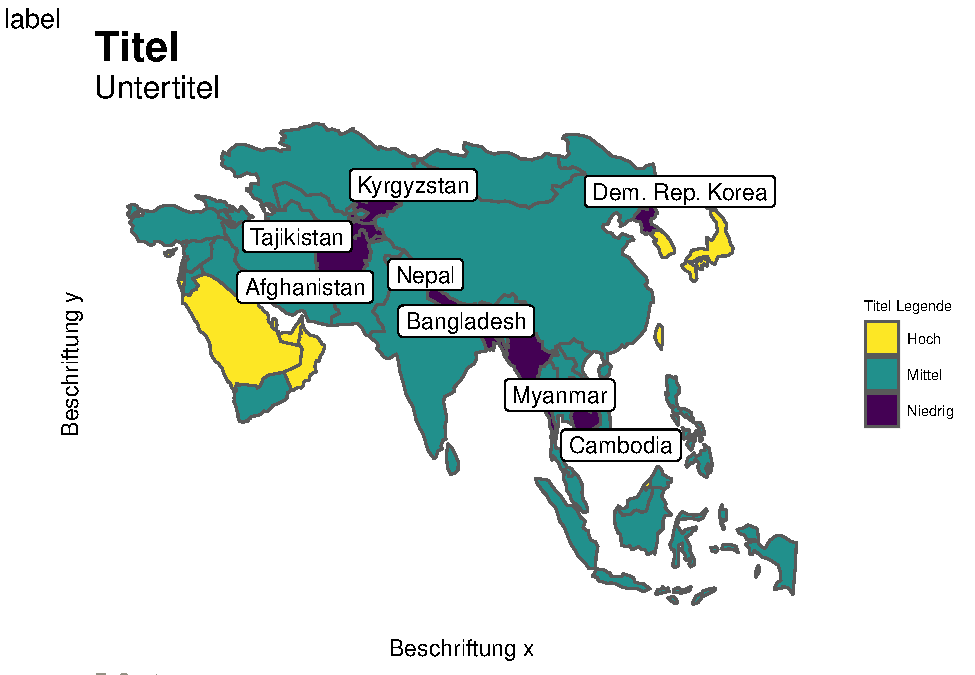
\includegraphics{ggplot2_files/figure-latex/unnamed-chunk-5-1.pdf}

\hypertarget{gemischtes-1-und-2-spalten-layout}{%
\section{Gemischtes 1 und 2 Spalten
Layout}\label{gemischtes-1-und-2-spalten-layout}}

\begin {multicols}{2}

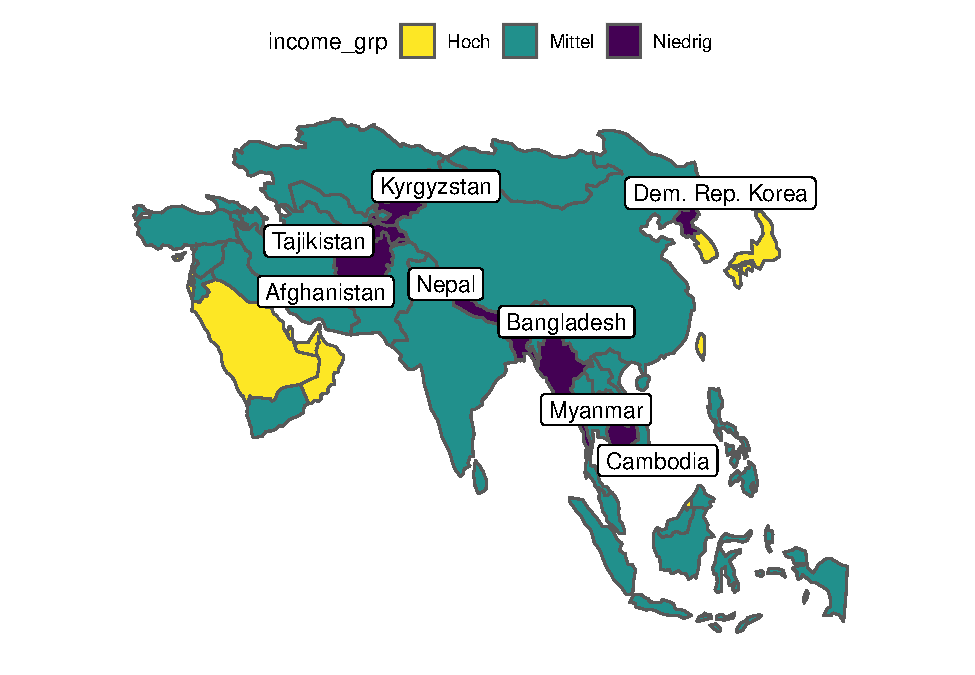
\includegraphics{ggplot2_files/figure-latex/unnamed-chunk-6-1.pdf} Lorem
ipsum dolor sit amet, consetetur sadipscing elitr, sed diam nonumy
eirmod tempor invidunt ut labore et dolore magna aliquyam erat, sed diam
voluptua. At vero eos et accusam et justo duo dolores et ea rebum.
\columnbreak

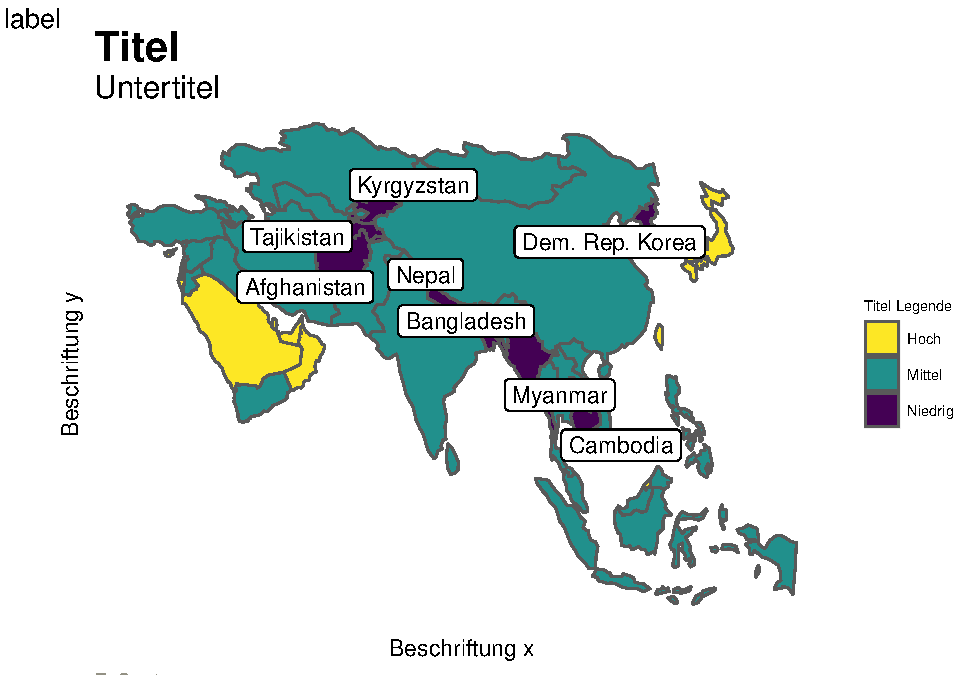
\includegraphics{ggplot2_files/figure-latex/unnamed-chunk-7-1.pdf} Lorem
ipsum dolor sit amet, consetetur sadipscing elitr, sed diam nonumy
eirmod tempor invidunt ut labore et dolore magna aliquyam erat, sed diam
voluptua. At vero eos et accusam et justo duo dolores et ea rebum.

\end {multicols}

\begin{verbatim}
## `geom_smooth()` using formula 'y ~ x'
\end{verbatim}

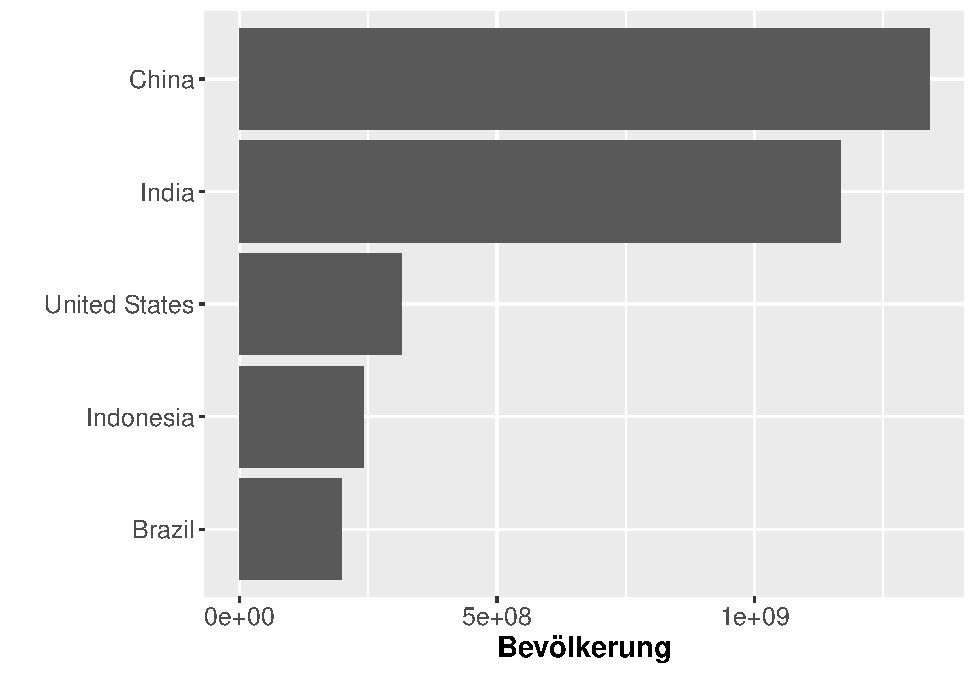
\includegraphics{ggplot2_files/figure-latex/unnamed-chunk-8-1.pdf}

\end{document}
